
% This LaTeX was auto-generated from MATLAB code.
% To make changes, update the MATLAB code and republish this document.

\documentclass{article}
\usepackage{graphicx}
\usepackage{color}

\sloppy
\definecolor{lightgray}{gray}{0.5}
\setlength{\parindent}{0pt}

\begin{document}

    
    
\subsection*{Contents}

\begin{itemize}
\setlength{\itemsep}{-1ex}
   \item ASSIGNMENT 2 - INTERPLANETARY FLYBY
   \item TIMES MATRIX COMPUTATION
   \item DEFINE ORBITS
   \item MAIN ROUTINE
   \item FLYBY
\end{itemize}


\subsection*{ASSIGNMENT 2 - INTERPLANETARY FLYBY}


\begin{verbatim}Planetes : Mars, Saturn, Neptune
(C) Collogrosso, Cuzzocrea, Lui - POLIMI SPACE AGENCY
WEB : https://github.com/fcuzzocrea/OrbitalMechanics2016\end{verbatim}
    \begin{verbatim}
clear
close all
clc

% File for saving datas
if exist(fullfile(cd, 'results_flyby.txt'), 'file') == 2
    delete(fullfile(cd, 'results_flyby.txt'))
end
filename = 'results_flyby.txt';
fileID = fopen(filename,'w+');
fprintf(fileID,'[ASSIGNMENT 2 : INTERPLANETARY FLYBY]\n');
fclose(fileID);

date =  [2016 1 1 12 0 0];
date = date2mjd2000(date);
\end{verbatim}


\subsection*{TIMES MATRIX COMPUTATION}

\begin{verbatim}
starting_departure_time = [2016 1 1 12 0 0];
final_departure_time = [2055 1 1 12 0 0];
fileID = fopen(filename,'a+');
fprintf(fileID,'[LOG] Mission Window : [%d %d %d %d %d %d] - [%d %d %d %d %d %d]\n',starting_departure_time,final_departure_time);
fclose(fileID);

% Conversion of departure dates from Gregorian calendar
% to modified Julian Day 2000.
date1_departure = date2mjd2000(starting_departure_time);
date2_departure = date2mjd2000(final_departure_time);

% Time of departure window vectors in days and seconds.
% One departure per month
t_dep = date1_departure : 100 : date2_departure ;
t_dep_sec = t_dep*86400;


% First and last arrival dates.
starting_arrival_time = [2016 1 1 12 0 0];
final_arrival_time = [2055 1 1 12 0 0];

% Conversion of arrival dates from Gregorian calendar
% to modified Julian Day 2000.
date1_arrival = date2mjd2000(starting_arrival_time);
date2_arrival = date2mjd2000(final_arrival_time);

% Time of arrival window vectors in days and seconds.
% One arrival per month
t_arr = date1_arrival: 100 : date2_arrival ;
t_arr_sec = t_arr*86400;

% Time of fligth computation.
TOF_matrix = tof_calculator (t_dep,t_arr);
for q = 1: numel(TOF_matrix)
    if TOF_matrix(q) <= 0
        TOF_matrix(q) = nan;
    end
end
\end{verbatim}


\subsection*{DEFINE ORBITS}

\begin{verbatim}
% Generic for plotting
ibody_mars = 4;
[kep_mars,ksun] = uplanet(date, ibody_mars);
[rx_mars, ry_mars, rz_mars, vx_mars, vy_mars, vz_mars] = int_orb_eq(kep_mars,ksun);

ibody_saturn = 6;
[kep_saturn,ksun] = uplanet(date, ibody_saturn);
[rx_saturn, ry_saturn, rz_saturn, vx_saturn, vy_saturn, vz_saturn] = int_orb_eq(kep_saturn,ksun);

ibody_neptune = 8;
[kep_neptune,ksun] = uplanet(date, ibody_neptune);
[rx_neptune, ry_neptune, rz_neptune, vx_neptune, vy_neptune, vz_neptune] = int_orb_eq(kep_neptune,ksun);

% From ephemeris compute position and velocity for the entire window
parfor i = 1 : length(t_dep)
    [kep_dep_vect_mars(i,:),~] = uplanet(t_dep(i),ibody_mars);
    [r_dep_vect_mars(i,:),v_dep_vect_mars(i,:)] = kep2car(kep_dep_vect_mars(i,:),ksun);
end

parfor i = 1 : length(t_dep)
    [kep_dep_vect_saturn(i,:),~] = uplanet(t_dep(i),ibody_saturn);
    [r_dep_vect_saturn(i,:),v_dep_vect_saturn(i,:)] = kep2car(kep_dep_vect_saturn(i,:),ksun);
end

parfor i = 1 : length(t_dep)
    [kep_dep_vect_neptune(i,:),~] = uplanet(t_dep(i),ibody_neptune);
    [r_dep_vect_neptune(i,:),v_dep_vect_neptune(i,:)] = kep2car(kep_dep_vect_neptune(i,:),ksun);
end
\end{verbatim}


\subsection*{MAIN ROUTINE}

\begin{verbatim}
% Preallocation
Dv_matrix_1 = zeros(size(t_dep));
Dv_matrix_2 = zeros(size(t_dep));
v_inf_matrix_1 = zeros(size(t_dep));
v_inf_matrix_2 = zeros(size(t_dep));
DV_Tensor = zeros(length(t_dep),length(t_dep),length(t_dep));

% Computation of the 3D-Tensor of deltav with 3 nested for cycles
for i = 1:length(t_dep)

    r_mars = r_dep_vect_mars(i,:);
    v_mars = v_dep_vect_mars(i,:);

    for j = 1:length(t_dep)

        tof_1 = TOF_matrix(i,j)*86400;

        if tof_1 > 0
            r_saturn = r_dep_vect_saturn(j,:);
            v_saturn = v_dep_vect_saturn(j,:);
            [~,~,~,~,VI_mars,VF_saturn,~,~] = lambertMR(r_mars,r_saturn,tof_1,ksun);
            dv1_mars = norm(VI_mars - v_mars);
            dv2_saturn = norm(v_saturn - VF_saturn);
            Dv_matrix_1(i,j) = abs(dv1_mars) + abs(dv2_saturn);
            v_inf_matrix_1(i,j) = dv1_mars;

            for k = 1:length(t_dep)

                tof_2 = TOF_matrix(j,k)*86400;

                if tof_2 > 0
                    r_neptune = r_dep_vect_neptune(k,:);
                    v_neptune = v_dep_vect_neptune(k,:);
                    [~,~,~,~,VI_saturn,VF_neptune,~,~] = lambertMR(r_saturn,r_neptune,tof_2,ksun);
                    dv1_saturn = norm(VI_saturn - v_saturn);
                    dv2_neptune = norm(v_neptune - VF_neptune);
                    Dv_matrix_2(j,k) = abs(dv1_saturn) + abs(dv2_neptune);
                    v_inf_matrix_2(j,k) = dv1_saturn;

                    dv_ga = abs(dv1_saturn - dv2_saturn);

                    DV_Tensor(i,j,k) = Dv_matrix_1(i,j) + dv_ga + Dv_matrix_2(j,k);

                else
                    Dv_matrix_2(j,k) = nan;
                    v_inf_matrix_2(j,k) = nan;
                    DV_Tensor(i,j,k) = nan;
                end
            end
        else
            Dv_matrix_1(i,j) = nan;
            v_inf_matrix_1(i,j) = nan;
            DV_Tensor(i,j,:) = nan;
        end
    end
end

% This is done due to fact that first row of output matrix is zeros
Dv_matrix_2(1,:) = nan;
v_inf_matrix_2(1,:) = nan;

% Find the minimum DV
DV_MIN = min(min(min(DV_Tensor)));
[row,column,depth] = ind2sub(size(DV_Tensor),find(DV_Tensor == DV_MIN));
fileID = fopen(filename,'a+');
fprintf(fileID,'[LOG] DELTAV MIN : \n',DV_MIN);
fclose(fileID);

% Find best arcs
r1_arc = r_dep_vect_mars(row,:);
r2_arc = r_dep_vect_saturn(column,:);
r3_arc = r_dep_vect_neptune(depth,:);

% Find correspondent TOFs
Dv_min_TOF_1 = (TOF_matrix(row,column)*86400);
Dv_min_TOF_2 = (TOF_matrix(column,depth)*86400);

[~,~,~,~,VI_arc1,VF_arc1,~,~] = lambertMR(r1_arc,r2_arc,Dv_min_TOF_1,ksun);
[~,~,~,~,VI_arc2,VF_arc2,~,~] = lambertMR(r2_arc,r3_arc,Dv_min_TOF_2,ksun);

[rx_arc_1, ry_arc_1, rz_arc_1, vx_arc_1, vy_arc_1, vz_arc_1] = intARC_lamb(r1_arc,...
    VI_arc1,ksun,Dv_min_TOF_1,86400);

[rx_arc_2, ry_arc_2, rz_arc_2, vx_arc_2, vy_arc_2, vz_arc_2] = intARC_lamb(r2_arc,...
    VI_arc2,ksun,Dv_min_TOF_2,86400);

% V infinity

v_saturn = v_dep_vect_saturn(column,:);

v_inf_min = (VF_arc1 - v_saturn );
v_inf_plus = (VI_arc2 - v_saturn);
\end{verbatim}


\subsection*{FLYBY}

\begin{verbatim}
r_soi_saturn = 1433449370*((5.683e26)/(1.989e30))^(2/5);

fileID = fopen(filename,'a+');
fprintf(fileID,'[LOG] Saturn SOI radius : \n',r_soi_saturn);
fclose(fileID);

if norm(v_inf_min) - norm(v_inf_plus) == 0
    disp('Powered gravity assist is not needed')
end

delta = acos(dot(v_inf_min,v_inf_plus)/(norm(v_inf_min)*norm(v_inf_plus)));
ksaturn = astroConstants(16);
f = @(r_p) delta - asin(1/(1+(r_p*norm(v_inf_min)^2/ksaturn))) - asin(1/(1+(r_p*norm(v_inf_plus)^2/ksaturn)));
r_p = fzero(f,700000) %Shitty IC because of shitty matlab solver
fileID = fopen(filename,'a+');
fprintf(fileID,'[LOG] Pericenter Radius of Hyperbola : \n',r_p);
fclose(fileID);

% Entering Hyperbola
e_min = 1 + (r_p*norm(v_inf_min)^2)/ksaturn;
delta_min = 2*(1/e_min);
DELTA_min = r_p*sqrt(1 + 2*(ksaturn/(r_p*norm(v_inf_min)^2)));
theta_inf_min = acos(-1/e_min);

% Exiting Hyperbola
e_plus = 1 + (r_p*norm(v_inf_plus)^2)/ksaturn;
delta_plus = 2*(1/e_plus);
DELTA_plus = r_p*sqrt(1 + 2*(ksaturn/(r_p*norm(v_inf_plus)^2))),
theta_inf_plus = acos(-1/e_plus);

%DeltaV Pericenter
vp_min = (DELTA_min*norm(v_inf_min))/(r_p);
vp_plus = (DELTA_plus*norm(v_inf_plus))/(r_p);
DELTA_VP = abs(vp_plus - vp_min);
fileID = fopen(filename,'a+');
fprintf(fileID,'[LOG] DeltaV to give : \n',DELTA_VP);
fclose(fileID);

figure
grid on
hold on
whitebg(figure(1), 'black')
plot3(rx_mars,ry_mars,rz_mars);
plot3(rx_neptune,ry_neptune,rz_neptune);
plot3(rx_saturn,ry_saturn,rz_saturn);
plot3(rx_arc_1, ry_arc_1, rz_arc_1,'y')
plot3(rx_arc_2, ry_arc_2, rz_arc_2,'w')
\end{verbatim}

        \color{lightgray} \begin{verbatim}
r_p =

     8.100819376509939e+05


DELTA_plus =

     1.866522492357928e+06

\end{verbatim} \color{black}
    
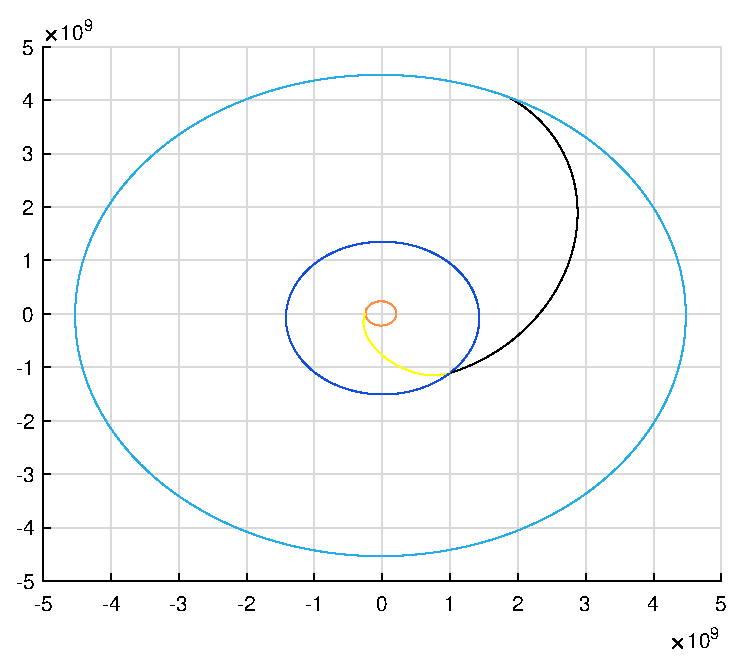
\includegraphics [width=4in]{saturn_express_flyby_01.eps}



\end{document}
    
